
\documentclass[]{article}

\title{Practica Ejercicios en R}

\date{}
\usepackage{braket}
\usepackage{bbold}
\usepackage{amsmath,amsfonts,amssymb,amsthm,booktabs}
\usepackage[margin=1.0in]{geometry}
\usepackage{graphicx}
\usepackage{chngcntr}
\usepackage{floatrow}
\usepackage{chngcntr}
\usepackage{hyperref}
\usepackage[spanish]{babel}
\usepackage[svgnames]{xcolor}

\usepackage{floatrow}
\floatsetup[table]{capposition=top}

\renewcommand{\spanishtablename}{Cuadro}
\usepackage{listings}
\usepackage[%
    font={small,sf},
    labelfont=bf,
    format=hang,    
    format=plain,
    margin=0pt,
    width=0.8\textwidth,
]{caption}
\usepackage[list=true]{subcaption}
\lstset{language=R,
    basicstyle=\small\ttfamily,
    stringstyle=\color{DarkGreen},
    otherkeywords={0,1,2,3,4,5,6,7,8,9},
    morekeywords={TRUE,FALSE},
    deletekeywords={data,frame,length,as,character},
    keywordstyle=\color{blue},
    commentstyle=\color{DarkGreen},
}

\counterwithin{figure}{section}
\renewcommand*{\figureautorefname}{Figura}


\usepackage[backend=biber]{biblatex}
\addbibresource{ref.bib}

\begin{document}
	\maketitle
	\begin{center}


\centerline{\textbf{TAREA 10} } 
\textbf{ }

\centerline{Alumno: } 
\centerline{Joaquín Arturo Velarde Moreno}


	\end{center}
	

\section{Introducción}
En este reporte hago uso del programa R 4.0.2 \cite{rproject} para poder resolver 3 problemas escogidos del libro de introducción a la probabilidad \cite{Material} y representare gráficamente los resultados para ver como se comportan las variables.


\section{Ejercicio 1, página 247}


Se saca una carta al azar de una baraja que consta de cartas numeradas del 2 al 10. Un jugador gana 1 dólar si el número de la carta es impar y pierde 1 dólar si el número es par. ¿Cuál es el valor esperado de sus ganancias?\\
\\
$E = \sum x *P(X=x)$ .\\
$E = (-1)P(x=-1) + 1(1)P(x=1)$.\\
$P(X=1) = \frac{4}{9}$ .\\
$P(X=-1) = \frac{4}{9}$ .\\
$E = (-1)(\frac{4}{9}) +(1)(\frac{4}{9})$. \\
$E = -\frac{1}{9}$ .\\
\\
Analíticamente, obtenemos que nuestro valor esperado es de $-\frac{1}{9}$ o $-0.11111111$.
Ahora pasaremos a aplicarlo en nuestro programa R,de acuerdo con nuestro problema tenemos una baraja con cartas numeradas del 2 al 10.
   \begin{lstlisting}
	Baraja <- c(2,3,4,5,6,7,8,9,10)
   \end{lstlisting}
de acuerdo con la instrucción debemos sacar una carta al azar de la baraja, para esto haremos uso de la función \textit{sample()}.
   \begin{lstlisting}
	carta  <- sample(Baraja, 1)
   \end{lstlisting}
Lo siguiente es validar si nuestro número es par o impar, para lo cual usaremos la operación módulo y lo guardaremos en un arreglo.
   \begin{lstlisting}
      if((carta %% 2) == 0)
      {
        Ganancias = - 1;
      }else {
        Ganancias =   1;
      }
	  ArregloGanancias = c(ArregloGanancias,Ganancias)

   \end{lstlisting}
   Por último, replicaremos nuestro proceso cuántas veces queramos para comprobar si se obtiene nuestro valor esperado.
      \begin{lstlisting}
  for(j in 1:Replicas)
  {
    Ganancias <- 0;
    for(i in 1:50)
    {
      carta  <- sample(Baraja, 1)
      if((carta %% 2) == 0)
      {
        Ganancias = - 1;
      }else {
        Ganancias =   1;
      }
      ArregloGanancias = c(ArregloGanancias,Ganancias)
    }
    Media = c(Media,mean(ArregloGanancias))
  }

      \end{lstlisting}
      Lo anterior nos dará como resultado que, a medida que el número de réplicas aumenta el valor de nuestra media, se aproxima más a $-\frac{1}{9}$ (\autoref{fig:casos}).
\begin{figure}[hbt!]
\centering
\subcaptionbox{Media del evento replicada 10 veces.}{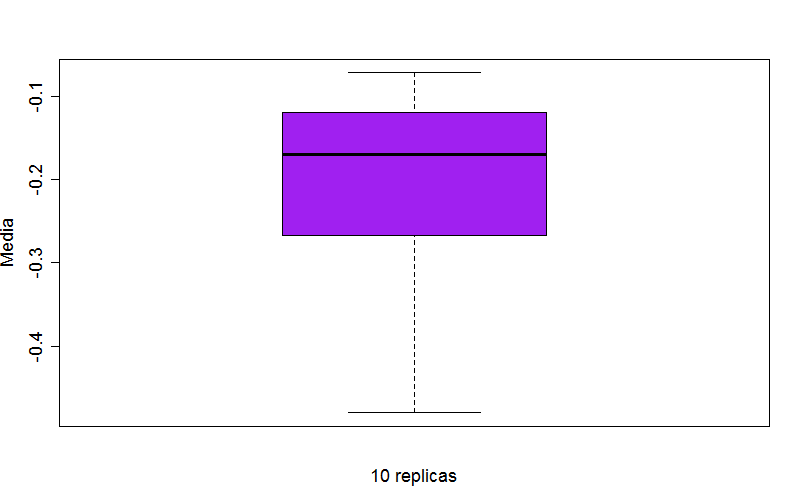
\includegraphics[width=0.3\textwidth]{Figuras/boxplot10.png}}%
\hfill
\subcaptionbox{Media del evento replicada 100 veces.}{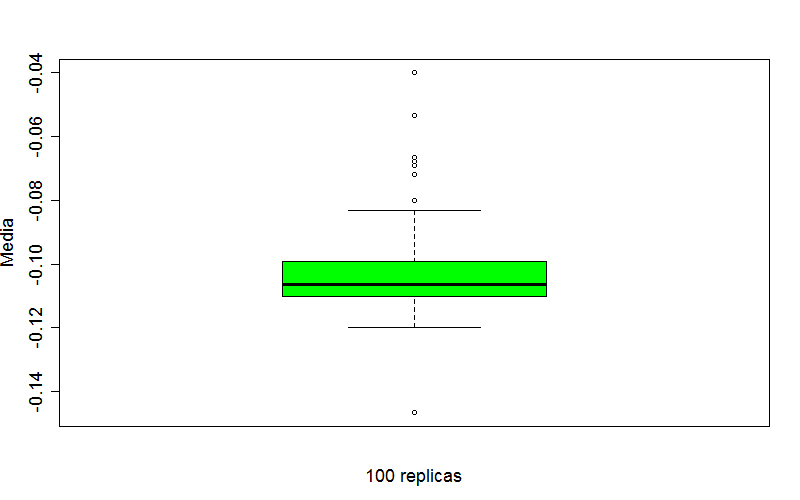
\includegraphics[width=0.3\textwidth]{Figuras/boxplot100.png}}%
\hfill
\subcaptionbox{Media del evento replicada 1000 veces.}{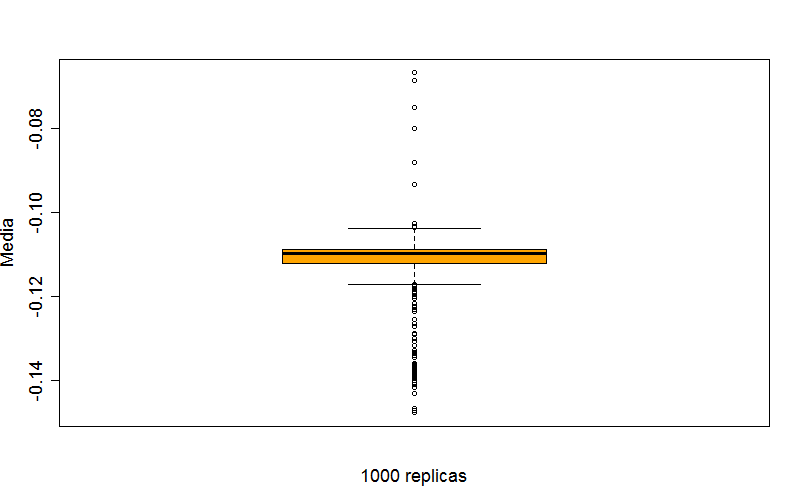
\includegraphics[width=0.3\textwidth]{Figuras/boxplot1000.png}}%
\hfill
\subcaptionbox{Media del evento replicada 10 veces.}{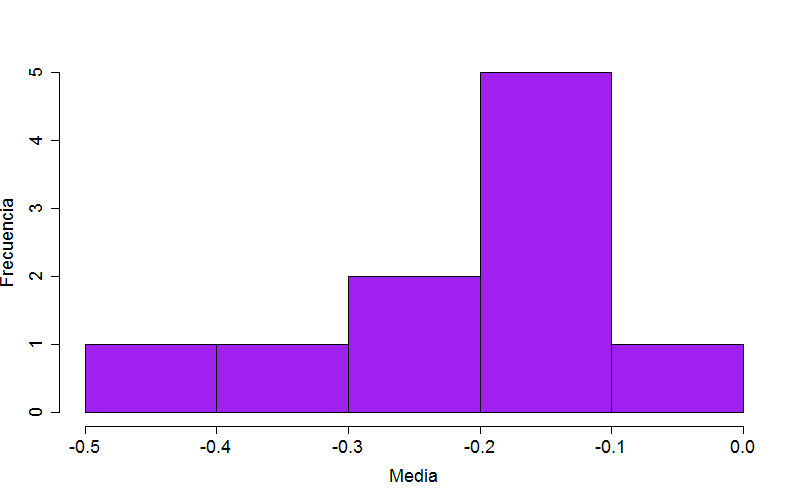
\includegraphics[width=0.3\textwidth]{Figuras/hist10.png}}%
\hfill
\subcaptionbox{Media del evento replicada 100 veces.}{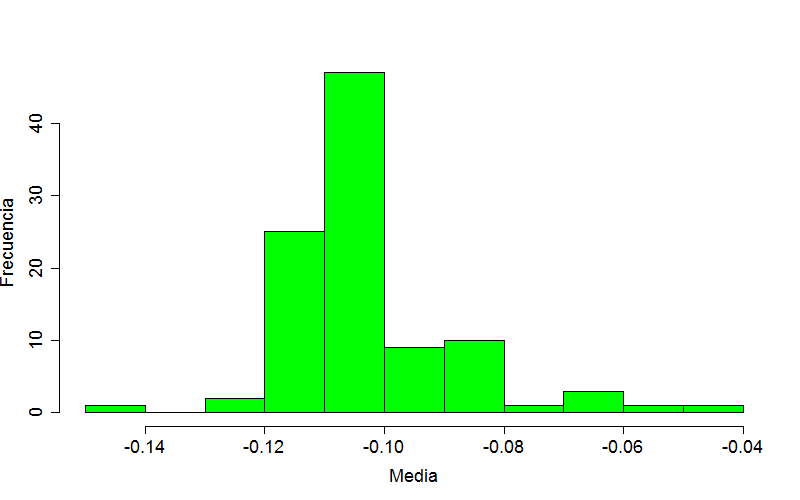
\includegraphics[width=0.3\textwidth]{Figuras/hist100.png}}%
\hfill
\subcaptionbox{Media del evento replicada 1000 veces.}{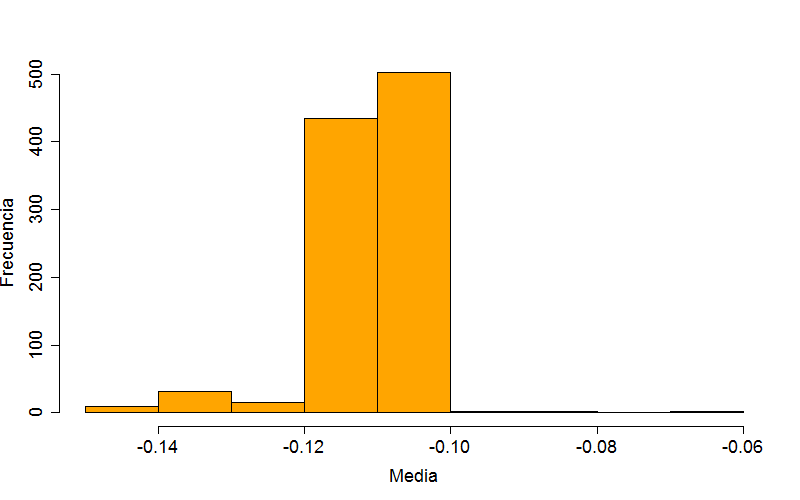
\includegraphics[width=0.3\textwidth]{Figuras/hist1000.png}}%
\hfill
\caption{Distribuciones de medias en los experimentos.}

\label{fig:casos}
\end{figure}




    
\section{Ejercicio 18, página 249}


Exactamente una de las seis llaves similares abre una puerta determinada. Si prueba las teclas, una tras otra, ¿cuál es la cantidad esperada de teclas que tendrá que probar antes de tener éxito?\\
\\
$E(X) = \sum_{x = 1}^{6} x * P(X = x)$.\\
$E(X) = \sum_{x = 1}^{6} x * \frac{1}{6}$.\\
$E(X) = (1+2+3+4+5+6)* \frac{1}{6}$.\\
$E(X) = 3.5$.\\
\\
Analíticamente, obtenemos que nuestro valor esperado es de $3.5$.
Para este ejercicio tomaremos un vector de 6 elementos para representar nuestras 6 llaves y estableceremos una llave correcta.
      \begin{lstlisting}
		Llaves         <- c(1:6)
		LlaveCorrecta  <- sample(Llaves, 1)

      \end{lstlisting}
Después, recorreremos nuestro vector en busca de la llave correcta, contando la veces que nos tomó encontrarla.
      \begin{lstlisting}
	Llaves         <- c(1:6)
	LlaveCorrecta  <- sample(Llaves, 1)
    for (LLave in LLaves) 
    {
      if(LLave == LLaveCorrecta)
      {
        break;
      }else{
        contador = contador + 1;
      }
    }
      \end{lstlisting}
Por último, calcularemos la media de las veces que nos tomó encontrarlas.
           \begin{lstlisting}
  for(i in 1:100)
  {
    LLaveCorrecta  <- sample(LLaves, 1)
    contador       <- 0;
    for (LLave in LLaves) 
    {
      if(LLave == LLaveCorrecta)
      {
        break;
      }else{
        contador = contador + 1;
      }
    }
    contadores = c(contadores,contador)
  }
  Medias  <- c(Medias,mean(contadores))
      \end{lstlisting}
      
 Para nuestra sorpresa, el valor de la media obtenido más frecuentemente es el de $2.5$ por lo que son necesarias más pruebas.
 \begin{figure}[hbt!]
\centering
\subcaptionbox{Frecuencia de medias.}{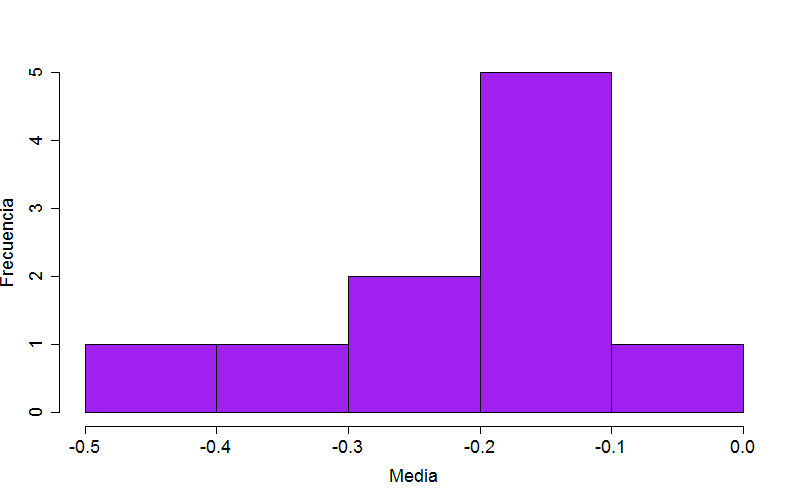
\includegraphics[width=0.4\textwidth]{Figuras/histllave.png}}%
\hfill
\subcaptionbox{Distribuciones de media.}{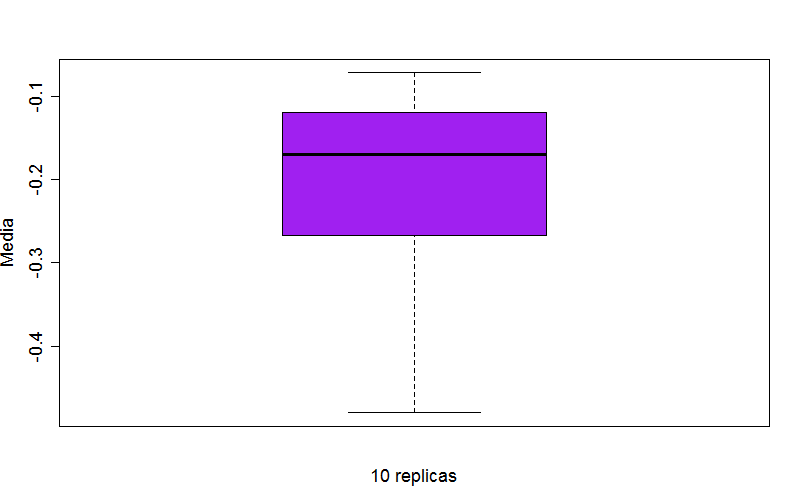
\includegraphics[width=0.4\textwidth]{Figuras/boxplotllave.png}}%
\hfill


\caption{Distribución de la media para el número de llaves necesarias en 10 eventos.}

\label{fig:casos2}
\end{figure}
     
\section{Ejercicio 1, página 263}
Se elige un número al azar del conjunto $ S = \{- 1, 0, 1\} $. Sea $ X $ el número elegido. Encuentre el valor esperado, la varianza y la desviación estándar de $ X $.\\
$E(X) = \sum_{x = 1}^{3} x * P(X = x)$.\\
$E(X) = \sum_{x = 1}^{3} x * \frac{1}{3}$.\\
$E(X) = (-1, 0, 1)* \frac{1}{3}$.\\
$E(X) = 0$.\\
Ahora para la varianza:
$\sigma^{2} = V(X) = E((x-E(x))^{2})$.\\
$\sigma^{2} = E((x-0)^{2})$.\\
$\sigma^{2} = E(x^{2})$.\\
$\sigma^{2} = \sum x^{2} * P(X^{2} = x^{2})$.\\
$\sigma^{2}  = (0 * \frac{1}{3}) + (1 * \frac{2}{3})$.\\
$\sigma^{2}  = \frac{2}{3}$.\\
Finalmente, la desviación estándar:
$\sigma = \sqrt{\frac{2}{3}}$.\\

Dado que, analíticamente conseguimos nuestro valor de la media como $0$, la varianza como $0,6$ y la desviación estándar como $0,81$, aplicaremos el ejercicio en R, para lo cual, primero necesitamos un arreglo que vaya de -1 a 1 y obtener un número al azar.
      \begin{lstlisting}
    Numeros   <- c(-1,0,1)
    Numero    <- sample(Numeros, 1)

      \end{lstlisting}
      
Realizaremos este proceso 100 veces y guardaremos nuestros resultados en un vector.
      \begin{lstlisting}
Numeros         <- c(-1,0,1)

  DistribucionNumeros <- c()
  for(i in 1:100)
  {
    Numero    <- sample(Numeros, 1)
    DistribucionNumeros <- c(DistribucionNumeros,Numero)
  }

      \end{lstlisting}
      
Por último, obtendremos la media, la varianza y la desviación estándar de cada uno y repetiremos este proceso 1000 veces para ver el resultado.

      \begin{lstlisting}
Numeros         <- c(-1,0,1)
for(j in 1:1000)
{
  DistribucionNumeros <- c()
  for(i in 1:100)
  {
    Numero    <- sample(Numeros, 1)
    DistribucionNumeros <- c(DistribucionNumeros,Numero)
  }
  ArrayMedias     = c(ArrayMedias,mean(DistribucionNumeros))
  ArrayVarianza   = c(ArrayVarianza,var(DistribucionNumeros))
  ArrayDestandar  = c(ArrayDestandar,sd(DistribucionNumeros))
}

      \end{lstlisting}
      
Con lo anterior, se muestra que nuestros valores se acercan a los obtenidos analíticamente \autoref{fig:casos3}.
 \begin{figure}[hbt!]
\centering
\subcaptionbox{Frecuencia de medias obteniendo en promedio $0$.}{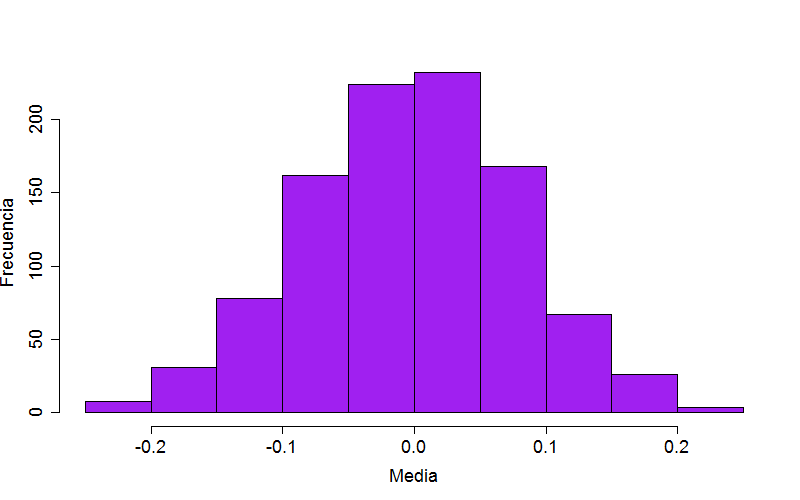
\includegraphics[width=0.3\textwidth]{Figuras/histmedia.png}}%
\hfill
\subcaptionbox{Frecuencia de la varianza obteniendo en promedio $0.6$.}{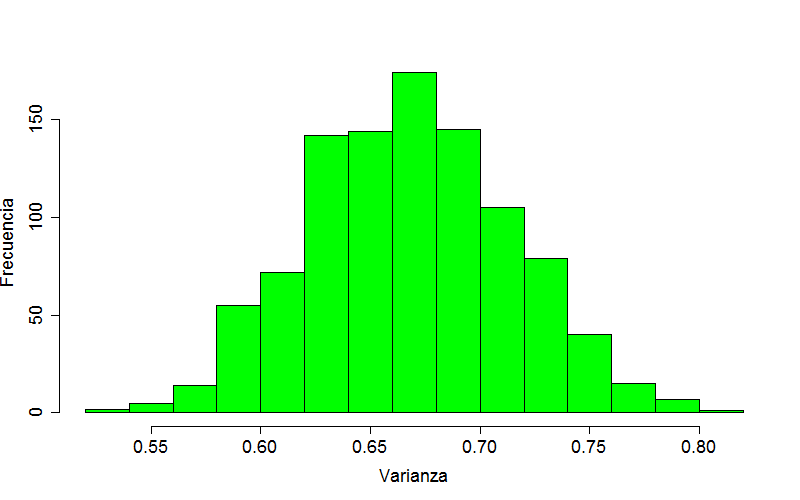
\includegraphics[width=0.3\textwidth]{Figuras/histvarianza.png}}%
\hfill
\subcaptionbox{Frecuencia de la desviación estándar obteniendo en promedio $0.81$.}{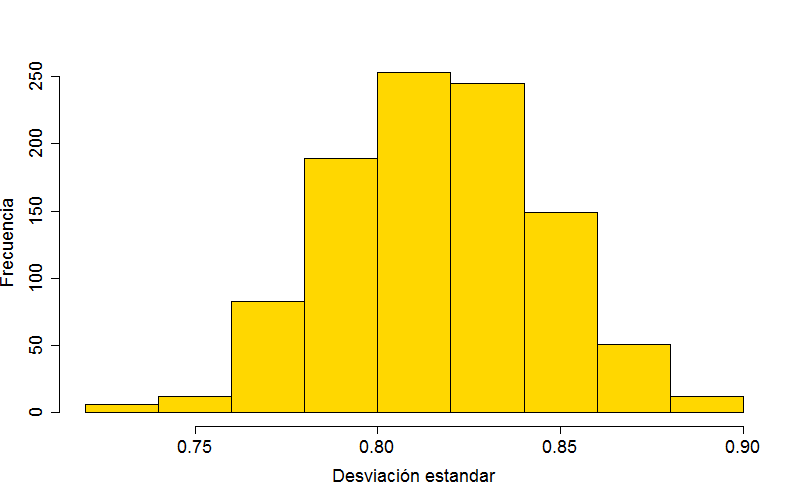
\includegraphics[width=0.3\textwidth]{Figuras/histDE.png}}%
\hfill

\caption{Frecuencias de la media, varianza y desviación estándar.}

\label{fig:casos3}
\end{figure} 
\hfill
\printbibliography[title={Referencias}]
\end{document}
